\documentclass[10pt,a4paper,onecolumn]{article}
% \usepackage[utf8]{inputenc}
\usepackage{marginnote}
\usepackage{graphicx}
\usepackage{xcolor}
\usepackage{authblk,etoolbox}
\usepackage{titlesec}
\usepackage{calc}
\usepackage{hyperref}
% \hypersetup{breaklinks=true,
%             bookmarks=true,
%             pdfauthor=
% {
%       Georgios Detorakis,
%   },
%             pdftitle=
% {
% [Re] A Generalized Linear Integrate-and-Fire Neural Model Produces Diverse
%         Spiking Behavior
% },
%             colorlinks=true,
%             citecolor=blue,
%             urlcolor=blue,
%             linkcolor=blue,
%             pdfborder={0 0 0}}
\urlstyle{same}
\usepackage{tcolorbox}
\usepackage{ragged2e}
\usepackage{fontspec}
\usepackage{fontawesome}
\usepackage{caption}
\usepackage{listings}
\lstnewenvironment{code}{\lstset{language=Haskell,basicstyle=\small\ttfamily}}{}

\usepackage{float,lscape}
\usepackage{xcolor,colortbl}
\usepackage{amssymb,amsmath,array,amsthm}
\usepackage{marvosym}
% \usepackage{makecell}
\usepackage{boldline}
\usepackage{bm,array}

\usepackage{adjustbox}


\newcommand{\Rm}[1]{\mathrm{#1}}

\newcolumntype{C}{>{\centering\arraybackslash}p{3.5em}}

\makeatletter
\newcommand{\thickhline}{%
    \noalign {\ifnum 0=`}\fi \hrule height 1pt
    \futurelet \reserved@a \@xhline
}
\newcolumntype{"}{@{\hskip\tabcolsep\vrule width 1pt\hskip\tabcolsep}}
\makeatother

\definecolor{Gray}{gray}{0.75}
\definecolor{LightGray}{gray}{0.95}



%\usepackage{fancyvrb}
%\VerbatimFootnotes
%\usepackage{graphicx}
%\usepackage{mdframed}
%\newmdenv[backgroundcolor=lightgray]{Shaded}


\usepackage{longtable,booktabs}

\usepackage[
  backend=biber,
%  style=alphabetic,
%  citestyle=numeric
]{biblatex}
\bibliography{bibliography.bib}



% --- Macros ------------------------------------------------------------------
\renewcommand*{\bibfont}{\small \sffamily}

\definecolor{red}{HTML}{CF232B}
\newcommand{\ReScience}{Re{\bfseries \textcolor{red}{Science}}}

\newtcolorbox{rebox}
   {colback=blue!5!white, colframe=blue!40!white,
     boxrule=0.5pt, arc=2pt, fonttitle=\sffamily\scshape\bfseries,
     left=6pt, right=20pt, top=6pt, bottom=6pt}

\newtcolorbox{repobox}
   {colback=red, colframe=red!75!black,
     boxrule=0.5pt, arc=2pt, left=6pt, right=6pt, top=3pt, bottom=3pt}

% fix for pandoc 1.14     
\newcommand{\tightlist}{%
  \setlength{\itemsep}{1pt}\setlength{\parskip}{0pt}\setlength{\parsep}{0pt}}

% --- Style -------------------------------------------------------------------
\renewcommand*{\bibfont}{\small \sffamily}
\renewcommand{\captionfont}{\small\sffamily}
\renewcommand{\captionlabelfont}{\bfseries}

\makeatletter
\renewcommand\@biblabel[1]{{\bf #1.}}
\makeatother

% --- Page layout -------------------------------------------------------------
\usepackage[top=3.5cm, bottom=3cm, right=1.5cm, left=1.5cm,
            headheight=2.2cm, reversemp, includemp, marginparwidth=4.5cm]{geometry}

% --- Section/SubSection/SubSubSection ----------------------------------------
\titleformat{\section}
  {\normalfont\sffamily\Large\bfseries}
  {}{0pt}{}
\titleformat{\subsection}
  {\normalfont\sffamily\large\bfseries}
  {}{0pt}{}
\titleformat{\subsubsection}
  {\normalfont\sffamily\bfseries}
  {}{0pt}{}
\titleformat*{\paragraph}
  {\sffamily\normalsize}


% --- Header / Footer ---------------------------------------------------------
\usepackage{fancyhdr}
\pagestyle{fancy}
%\renewcommand{\headrulewidth}{0.50pt}
\renewcommand{\headrulewidth}{0pt}
\fancyhead[L]{\hspace{-1cm}
\includegraphics[width=4.0cm]{rescience-logo.pdf}}
\fancyhead[C]{}
\fancyhead[R]{} 
\renewcommand{\footrulewidth}{0.25pt}

\fancyfoot[L]{\hypersetup{urlcolor=red}
              \sffamily \ReScience~$\vert$
              \href{http://rescience.github.io}{rescience.github.io}
              \hypersetup{urlcolor=blue}}
\fancyfoot[C]{\sffamily 1 - \thepage}
\fancyfoot[R]{\sffamily Sep 2015 $\vert$
                        Volume \textbf{1} $\vert$
                        Issue \textbf{1}}
\pagestyle{fancy}
\makeatletter
\let\ps@plain\ps@fancy
\fancyheadoffset[L]{4.5cm}
\fancyfootoffset[L]{4.5cm}

% --- Title / Authors ---------------------------------------------------------
% patch \maketitle so that it doesn't center
\patchcmd{\@maketitle}{center}{flushleft}{}{}
\patchcmd{\@maketitle}{center}{flushleft}{}{}
% patch \maketitle so that the font size for the title is normal
\patchcmd{\@maketitle}{\LARGE}{\LARGE\sffamily}{}{}
% patch the patch by authblk so that the author block is flush left
\def\maketitle{{%
  \renewenvironment{tabular}[2][]
    {\begin{flushleft}}
    {\end{flushleft}}
  \AB@maketitle}}
\makeatletter
\renewcommand\AB@affilsepx{ \protect\Affilfont}
%\renewcommand\AB@affilnote[1]{{\bfseries #1}\hspace{2pt}}
\renewcommand\AB@affilnote[1]{{\bfseries #1}\hspace{3pt}}
\makeatother
\renewcommand\Authfont{\sffamily\bfseries}
\renewcommand\Affilfont{\sffamily\small\mdseries}
\setlength{\affilsep}{1em}

\LetLtxMacro{\OldIncludegraphics}{\includegraphics}
\renewcommand{\includegraphics}[2][]{\OldIncludegraphics[width=12cm, #1]{#2}}


% --- Document ----------------------------------------------------------------
\title{[Re] A Generalized Linear Integrate-and-Fire Neural Model Produces
            Diverse Spiking Behaviors}

    \usepackage{authblk}
                        \author[1]{Georgios Detorakis}
                            \affil[1]{Department of Cognitive Sciences, UC Irvine,
                            Irvine, CA, USA}
            
\date{\vspace{-5mm}
      \sffamily \small
      \href{mailto:corresponding-author@mail.com}{gdetorak@uci.edu \\
      gdetor@protonmail.com}}


\setlength\LTleft{0pt}
\setlength\LTright{0pt}


\begin{document}
\maketitle

\marginpar{
  %\hrule
  \sffamily\small
  %\vspace{2mm}
  {\bfseries Editor}\\
  Name Surname\\

  {\bfseries Reviewers}\\
        Name Surname\\
        Name Surname\\
  
  {\bfseries Received}  Sep, 1, 2015\\
  {\bfseries Accepted}  Sep, 1, 2015\\
  {\bfseries Published} Sep, 1, 2015\\

  {\bfseries Licence}   \href{http://creativecommons.org/licenses/by/4.0/}{CC-BY}

  \begin{flushleft}
  {\bfseries Competing Interests:}\\
  The author has declared that no competing interests exist.
  \end{flushleft}

  \hrule
  \vspace{3mm}

  \hypersetup{urlcolor=white}
  
    \vspace{-1mm}
  \begin{repobox}
    \bfseries\normalsize
      \href{http://github.com/rescience/rescience-submission/article}{\faGithubAlt~Article repository}
  \end{repobox}
      \vspace{-1mm}
  \begin{repobox}
    \bfseries\normalsize
      \href{http://github.com/rescience/rescience-submission/code}{\faGithubAlt~Code repository}
  \end{repobox}
        \hypersetup{urlcolor=blue}
}

\begin{rebox}
\sffamily {\bfseries A reference implementation of}
\small
\begin{flushleft}
\begin{itemize}
    \item[→] A Generalized Linear Integrate-and-Fire Neural Model Produces
        Diverse Spiking Behaviors, Stefan Mihalas and Ernst Niebur, Neural
        Computation 21, 704--718, 2009.
  \end{itemize}\par
\end{flushleft}
\end{rebox}


\section{Introduction}\label{introduction}

Integrate-and-fire neurons are being used extensively in the field of 
neuroscience for modeling spiking behaviors~\cite{dayan:2001}. In this work we
provide a reference implementation of~\cite{mihalas:2009}, where the authors
have introduced a generalization of the leaky integrate-and-fire neuron model. 
The Mihalas-Niebur Neuron (MNN) model is a linear integrate-and-fire neuron
model capable of expressing a rich spiking behavior based on a set of 
parameters.

An MNN model expresses tonic and phasic spiking, class $1$ and $2$, spike
frequency adaptation, accommodation, threshold variability, rebound spike,
integrator, input bistability, hyperpolarizing spiking and bursting, tonic,
phasic and rebound bursting, mixed mode, afterpotentials, basal bistability, 
preferred frequency and spike latency. 
Due to its simplicity, the MNN model has been used in neuromorphic 
implementations such as~\cite{folowosele:2011}. 

The model consists of linear differential equations, which describe the membrane
and threshold potentials and internal currents. All the results provided in 
\cite{mihalas:2009} have been obtained by using only two internal currents and
thus we use the exact same number of internal currents in this work. The
subthreshold dynamics are defined by a set of linear ordinary differential 
equations, while an instantaneous threshold potential controls when the neuron
fires an action potential (spike) in a dynamic way. The ability of the MNN 
model to generate 
such a diverse spiking behavior is due to the complex update rules. In this 
work the MNN model has been implemented in Python (version 3.6.1) using 
Numpy (version 1.13.1) and Matplotlib (version 2.0.2) packages. 



\section{Methods}\label{methods}

In order to implement the model described in \cite{mihalas:2009}, we discretized
the dynamical system using the forward Euler integration scheme. The time step
is fixed to $0.1\, \Rm{ms}$ for all the simulations, and the total simulation
time $t_f$ varies according to figure 1 of the original paper. Our
implementation differs from the one in the original paper, since in
\cite{mihalas:2009}, authors numerically solve equation $3.5$ (algebraic 
equation) under the constraint imposed by inequality $3.4$ and thus they
compute the spike times. On the other hand, in this work we directly compute
numerically the solution of the dynamical system defined by equations $2.1$
and $2.2$ in \cite{mihalas:2009} (see tables~\ref{table:2} and~\ref{table:3}). 

We provide all equations and parameters of the model in tables as it has been 
suggested by~\cite{nordlie:2009}. 
Table~\ref{table:1} provides the summary of the model. Tables~\ref{table:2}
and~\ref{table:3} give the subthreshold dynamics (differential equations) 
describing the membrane and the threshold potentials as well as the two internal
currents and the update rules. The parameters for all the simulations are given
in table~\ref{table:4}, while the external current intensities and pulse
duration are provided in table~\ref{table:5}. The parameters in this work are 
exactly the same used in the original paper (table 1, pg. $711$). We had to 
infer the time intervals and the total simulation times for the pulses since
they are not given explicitly in the original paper. Thus, we extracted the
time intervals from figure $1$ of \cite{mihalas:2009} by visual inspection. 
The initial conditions are given in table~\ref{table:6}. 

All simulations ran on a Dell OptiPlex $7040$, equipped with a sixth
generation i$7$ processor, $16\, \Rm{GB}$ of physical memory and running Arch
Linux (x$86\_64$). The total execution time of all simulations was $2.41$
seconds and the peak consumed memory was $162\, \Rm{MB}$\footnote{Python memory
profiler used (\url{https://pypi.python.org/pypi/memory_profiler}).}\@. 

%%
\begin{table}[!htbp]
    \centering
    \begin{tabular}{ll}
        \thickhline
        \multicolumn{2}{c}{Model Summary} \\\thickhline
        \rowcolor{Gray}
        Populations  & No population -- single neuron model \\\rowcolor{LightGray}
        Topology     & -- \\ \rowcolor{Gray}
        Connectivity & -- \\ \rowcolor{LightGray}
        Neuron Model & Linear Integrate-and-Fire Neuron \\\rowcolor{Gray}
        Channel Models & Linear, first order ODEs  \\ \rowcolor{LightGray}
        Synapse Model & -- \\ \rowcolor{Gray}
        Plasticity & -- \\ \rowcolor{LightGray}
        Input & Constant current or rectangular pulses \\\rowcolor{Gray}
        Measurements & Membrane potential, phase plane \\
        \thickhline
    \end{tabular}
    \caption{{\bfseries \sffamily Summary of the model}} 
    \label{table:1}
\end{table}
%%  

%%
\begin{table}[!htbp]
    \centering
    \begin{tabular}{p{3.5cm}ll}
        \thickhline
        \multicolumn{2}{c}{Neuron Model} \\\thickhline
        \rowcolor{Gray}
        Name  &  Mihalas-Niebur Neuron (MNN) \\ \rowcolor{LightGray}
        Type  &  Linear Leaky Integrate-and-Fire Neuron  \\ \rowcolor{Gray}
        Membrane Potential & $
            \begin{aligned}
                \frac{\Rm{d}V(t)}{\Rm{d}t} &= \frac{1}{C} \Big(I_e + I_1 + I_2 - G(V(t) -
                E_L)  \Big)
            \end{aligned}$ \\ \rowcolor{LightGray}
        Instantaneous Threshold Potential  & $
            \begin{aligned}
                \frac{\Rm{d}\Theta(t)}{\Rm{d}t} &= a(V(t) - E_L) - b(\Theta(t) -
                \Theta_{\infty}) 
            \end{aligned} $
            \\ \rowcolor{Gray}
        Internal Currents & $
            \begin{aligned}
                \frac{\Rm{d}I_{1}(t)}{\Rm{d}t} &= -k_1I_1(t)\\
                \frac{\Rm{d}I_{2}(t)}{\Rm{d}t} &= -k_2I_2(t) \\
            \end{aligned} $
    \end{tabular}
    \caption{{\bfseries \sffamily Description of the subthreshold dynamics of
    Mihalas-Niebur neuron model.} $V(t)$ and $\Theta(t)$ are the membrane and 
    threshold potentials, respectively. $E_L$ and $\Theta_{\infty}$ are the
    reversal potentials for the membrane and the threshold variables,
    respectively. $a, b, k_1, k_2$ and $G$ are constant parameters. $I_e$ is
    the external current applied on the neuron model.} 
    \label{table:2}
\end{table}
%%

\begin{table}[!htbp]
    \centering
    \begin{tabular}{cc}
        \thickhline
        \multicolumn{2}{c}{Update rules} \\ \thickhline
        Variable & Rule  \\ \rowcolor{Gray}
        $V(t)$ & $V_r$  \\ \rowcolor{LightGray}
        $\Theta(t)$ & $\max\{\Theta_r, \Theta(t) \}$ \\ \rowcolor{Gray}
        $I_1(t)$ & $R_1 \times I_1(t) + A_1$ \\ \rowcolor{LightGray} 
        $I_2(t) $ & $R_2 \times I_2(t) + A_2$ \\\thickhline
    \end{tabular}
    \caption{{\bfseries \sffamily Update rules.} $V_r$ and $\Theta_r$
    are the reset values for the membrane and threshold potentials,
    respectively. $R_1, R_2, A_1$ and $A_2$ are constants.}
    \label{table:3}
\end{table}
%%  

%%
\begin{table}[!htbp]
    \centering
    \begin{tabular}{CCCCC}
        \thickhline
        \multicolumn{5}{c}{Model Parameters} \\\thickhline
           \begin{tabular}[x]{@{}c@{}} Figure \\  \end{tabular}
         & \begin{tabular}[x]{@{}c@{}} $a$ \\ $(\Rm{s^{-1}})$ \end{tabular}
         & \begin{tabular}[x]{@{}c@{}} $A_1/C$ \\ $(\Rm{V/s})$ \end{tabular}
         & \begin{tabular}[x]{@{}c@{}} $A_2/C$ \\ $(\Rm{V/s})$ \end{tabular}& 
           \begin{tabular}[x]{@{}c@{}} $t_f$ \\ $(\Rm{s})$ \end{tabular} \\
        \thickhline
        1A & $0$ & $0$ & $0$ & $0.2$ \\\rowcolor{Gray}
        1B & $0$ & $0$ & $0$ & $0.5$  \\\rowcolor{LightGray}
        1C & $5$ & $0$ & $0$ & $0.2$ \\\rowcolor{Gray}
        1D & $5$ & $0$ & $0$ & $0.5$ \\\rowcolor{LightGray}
        1E & $5$ & $0$ & $0$ & $1.0$ \\\rowcolor{Gray}
        1F & $5$ & $0$ & $0$ & $0.4$ \\\rowcolor{LightGray}
        1G & $5$ & $0$ & $0$ & $1.0$  \\\rowcolor{Gray}
        1H &  $5$ & $0$ & $0$ & $0.3$ \\\rowcolor{LightGray}
        1I & $5$  & $0$ & $0$ & $0.4$ \\\rowcolor{Gray}
        1J & $5$ & $0$ & $0$ & $1.0$ \\\rowcolor{LightGray}
        1K & $30$ & $0$ & $0$ & $0.4$ \\\rowcolor{Gray}
        1L & $30$  & $10$ & $-0.6$ & $0.4$ \\\rowcolor{LightGray}
        1M & $5$ & $10$ & $-0.6$ & $0.5$ \\\rowcolor{Gray}
        1N & $5$ & $10$ & $-0.6$ & $0.5$ \\\rowcolor{LightGray}
        1O & $5$ & $10$ & $-0.6$ & $1.0$ \\\rowcolor{Gray}
        1P & $5$  & $5$ & $-0.3$ & $0.5$ \\\rowcolor{LightGray}
        1Q & $5$  & $5$ & $-0.3$ & $0.2$ \\\rowcolor{Gray}
        1R & $0$ & $8$ & $-0.1$ & $0.2$ \\\rowcolor{LightGray}
        1S & $5$ & $-3$ & $0.5$ & $0.8$ \\\rowcolor{Gray}
        1T &  $-80$ & $0$ & $0$ & $0.05$ \\
        \thickhline
        \multicolumn{5}{l}{Common Parameters} \\\rowcolor{LightGray}
        \thickhline
        \multicolumn{5}{p{22.5em}}{
            $b = 10\, \Rm{s^{-1}}$, $G/C = 50\, \Rm{s^{-1}}$,
            $k_1 = 200\, \Rm{s^{-1}}$, $k_2 = 20\, \Rm{s^{-1}}$,
            $\Theta_{\infty} = -0.05\, \Rm{V}$,
            $R_1 = 0$, $R_2 = 1$, $E_l = -0.07\, \Rm{V}$,
            $V_r = -0.07\, \Rm{V}$, $\Theta_r = -0.06\, \Rm{V}$.
        }
        \\\thickhline
    \end{tabular}
    \caption{{\bfseries \sffamily Simulation Parameters}  }
    \label{table:4}
\end{table}
%%

\vspace{-1cm}

%%
\begin{table}[!htbp]
    \centering
    \begin{tabular}{CCp{28.2em}}
        \thickhline
        \multicolumn{3}{c}{Model Parameters} \\ \thickhline
        Figure & Type & $I_e/C (\Rm{V/s})$  \\
        \thickhline
        1A & 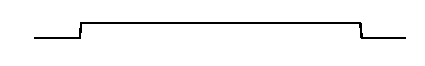
\includegraphics[width=0.1\textwidth]{figs/const.pdf} & $1.5$ \\\rowcolor{Gray}
        1B & 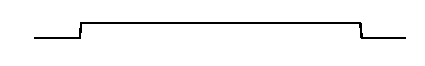
\includegraphics[width=0.1\textwidth]{figs/const.pdf} & $1 + 10^{-6}$ \\\rowcolor{LightGray}
        1C & 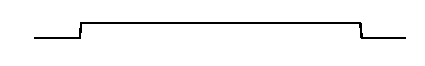
\includegraphics[width=0.1\textwidth]{figs/const.pdf} & $2$ \\\rowcolor{Gray}
        1D &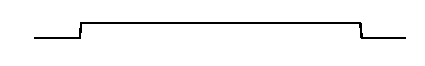
\includegraphics[width=0.1\textwidth]{figs/const.pdf} & $1.5$ \\\rowcolor{LightGray}
        1E &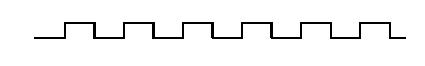
\includegraphics[width=0.1\textwidth]{figs/pulse.pdf} & 
              $1.5 (0.1 \Rm{s}),\, 0 (0.5\Rm{s}),\, 0.5 (0.1\Rm{s}),\, 1
              (0.1\Rm{s}),\, 1.5 (0.1\Rm{s}),\, 0 (0.1 \Rm{s})$
              \\\rowcolor{Gray}
        1F &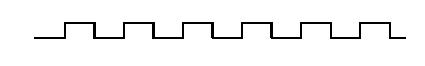
\includegraphics[width=0.1\textwidth]{figs/pulse.pdf} & $1.5 (0.02
        \Rm{s}),\, 0 (0.18 \Rm{s}),\, -1.5 (0.025 \Rm{s}),\, 0 (0.025
        \Rm{s}),\, 1.5 (0.025 \Rm{s}),\, 0 (0.125 \Rm{s})$
        \\\rowcolor{LightGray} 
        1G & 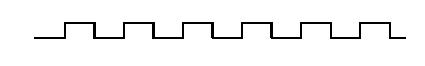
\includegraphics[width=0.1\textwidth]{figs/pulse.pdf} & $0 (0.05
        \Rm{s}),\, -3.5 (0.756 \Rm{s}),\, 0 (0.194 \Rm{s})$ \\\rowcolor{Gray} 
        1H & 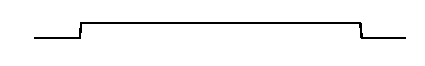
\includegraphics[width=0.1\textwidth]{figs/const.pdf} & $2(1 +
        10^{-6})$ \\\rowcolor{LightGray}
        1I & 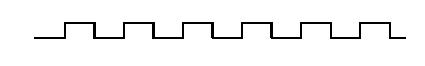
\includegraphics[width=0.1\textwidth]{figs/pulse.pdf} & 
        \begin{tabular}[x]{@{}c@{}} 
        $1.5 (0.02 \Rm{s}),\, 0 (0.01 \Rm{s}),\, 1.5 (0.02 \Rm{s}),\,
            0 (0.25 \Rm{s}),\, 1.5 (0.02 \Rm{s}),\, 0 (0.02 \Rm{s}) $\\
            $ 1.5 (0.02 \Rm{s}),\, 0 (0.04 \Rm{s})$ 
        \end{tabular}
            \\\rowcolor{Gray}
        1J & 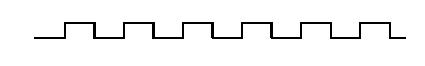
\includegraphics[width=0.1\textwidth]{figs/pulse.pdf} & $1.5 (0.1
        \Rm{s}),\, 1.7 (0.4 \Rm{s}),\, 1.5 (0.1 \Rm{s}),\, 1.7 (0.4 \Rm{s})$
        \\\rowcolor{LightGray}
        1K & 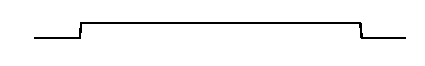
\includegraphics[width=0.1\textwidth]{figs/const.pdf} & $-1$  \\\rowcolor{Gray}
        1L & 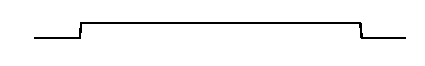
\includegraphics[width=0.1\textwidth]{figs/const.pdf} & $-1$ \\\rowcolor{LightGray}
        1M & 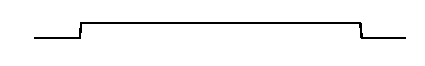
\includegraphics[width=0.1\textwidth]{figs/const.pdf} & $2$ \\\rowcolor{Gray}
        1N & 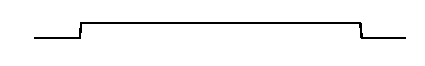
\includegraphics[width=0.1\textwidth]{figs/const.pdf} & $1.5$  \\\rowcolor{LightGray}
        1O &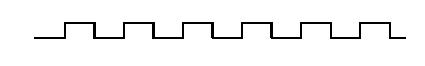
\includegraphics[width=0.1\textwidth]{figs/pulse.pdf} & $0 (0.1 
        \Rm{s}),\, -3.5 (0.5 \Rm{s}),\, 0 (0.4 \Rm{s})$ \\\rowcolor{Gray}
        1P & 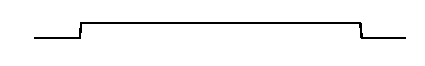
\includegraphics[width=0.1\textwidth]{figs/const.pdf} & $2$ \\\rowcolor{LightGray}
        1Q & 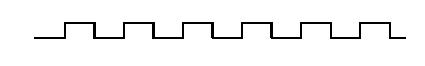
\includegraphics[width=0.1\textwidth]{figs/pulse.pdf} & $2 (0.015
        \Rm{s}),\, 0 (0.185 \Rm{s})$  \\\rowcolor{Gray}
        1R & 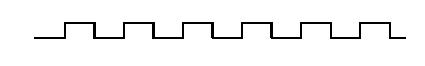
\includegraphics[width=0.1\textwidth]{figs/pulse.pdf}& $5 (0.01
        \Rm{s}),\, 0 (0.09 \Rm{s}),\, 5 (0.01 \Rm{s}),\, 0 (0.09 \Rm{s})$
        \\\rowcolor{LightGray}
        1S & 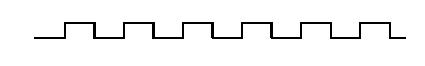
\includegraphics[width=0.1\textwidth]{figs/pulse.pdf}&
        \begin{tabular}[x]{@{}c@{}} 
            $5 (0.005 \Rm{s}),\, 0 (0.005 \Rm{s}),\, 4 (0.005 \Rm{s}),\, 0 (0.385 \Rm{s}),\,
            5 (0.005 \Rm{s}),\, 0 (0.045 \Rm{s}) $\\
            $4 (0.005\Rm{s}),\, 0 (0.345 \Rm{s}) $
        \end{tabular}
        \\\rowcolor{Gray}
        1T & 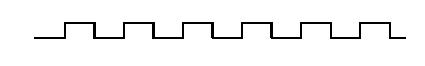
\includegraphics[width=0.1\textwidth]{figs/pulse.pdf} & $8 (0.002 \Rm{s}),\, 0 (0.048 \Rm{s})$ \\
        \thickhline
    \end{tabular}
    \caption{{\bfseries \sffamily External current.} This table provides the
    external current for each panel in Figure~\ref{fig:1}. There are two types
    of external currents, constants and pulses. In the case of pulses the
    duration of each pulse is given in seconds along with its intensity.
    }
    \label{table:5}
\end{table}
%%
\vspace{-2cm}
%%
\begin{table}[!htbp]
    \centering
    \begin{tabular}{cc}
        \thickhline
        \multicolumn{2}{c}{Initial Conditions} \\ \thickhline
        Variable & Initial Value  \\ 
        \rowcolor{Gray}
        $V(t)$ & $-0.07\, \Rm{V}$ / $-0.03\, \Rm{V}$ (Figure 1H) \\ \rowcolor{LightGray}
        $\Theta(t)$ & $-0.05\, \Rm{V}$ / $-0.03\, \Rm{V}$ (Figure 1H) \\ \rowcolor{Gray}
        $I_1(t)$ & $0.01\, \Rm{V}$ \\ \rowcolor{LightGray} 
        $I_2(t) $ & $0.001\, \Rm{V}$ \\ \thickhline
    \end{tabular}
    \caption{{\bfseries \sffamily Initial conditions.} In all simulations
    have been used the same initial conditions, except from the one 
    illustrated in Figure~\ref{fig:1}H.}
    \label{table:6}
\end{table}
%%  

\clearpage

\section{Results}\label{results}

All three figures from the original article have been successfully replicated.
All the different spiking behaviors of the model are illustrated in 
Figure~\ref{fig:1}, where the black solid line indicates the membrane potential
($V(t)$), the red dashed line illustrates the instantaneous threshold potentials
($\Theta(t)$), and the gray line shows the input to the neuron ($I_e/C$). 
The $x$-axis scales in all panels are exactly the same as in the original
paper (indicating the total simulation time ($t_f$), while the $y$-axis scale 
differs from the one in the original paper. In this work the $y$-axis scale
is the same same for all the subplots ($[-95, -25]\, \Rm{mV}$), except for
panels G and O ($[-145, -25]\, \Rm{mV}$).

Figures~\ref{fig:2} and~\ref{fig:3} depict the phase space of the phasic
spiking ($V(t)$ and $\Theta(t)$) and phasic bursting ($V(t)$,
$I_1(t)$, and $I_2(t)$). In both figures the blue curves and the black dots 
indicate the trajectory of the system and spike events, respectively.
In Figure~\ref{fig:2} the gray arrows show the evolution of the system
(vector field of the system). Figure~\ref{fig:3} has a different orientation 
from the original one but both illustrate the same trajectories and spike 
events of the system. 
All the figures express the same qualitative behavior as the original
figures in~\cite{mihalas:2009}.

\begin{figure}[htpb!]
    \centering
    \includegraphics[width=0.9\textwidth]{figs/Figure01.pdf}
    \caption{{\bfseries \sffamily Neural responses of MNN.} Black solid lines
    indicate the membrane potential ($V(t)$), the red dashed lines show the
    threshold potentials ($\Theta(t)$), and the gray lines the external
    currents applied on each case.
    {\bfseries \sffamily A} tonic spiking,
    {\bfseries \sffamily B} class $1$,
    {\bfseries \sffamily C} spike frequency adaptation,
    {\bfseries \sffamily D} phasic spiking,
    {\bfseries \sffamily E} accommodation,
    {\bfseries \sffamily F} threshold variability,
    {\bfseries \sffamily G} rebound spike,
    {\bfseries \sffamily H} class $2$,
    {\bfseries \sffamily I} integrator,
    {\bfseries \sffamily J} input bistability,
    {\bfseries \sffamily K} hyperpolarization induced spiking,
    {\bfseries \sffamily L} hyperpolarization induced bursting,
    {\bfseries \sffamily M} tonic bursting,
    {\bfseries \sffamily N} phasic bursting,
    {\bfseries \sffamily O} rebound burst,
    {\bfseries \sffamily P} mixed mode,
    {\bfseries \sffamily Q} afterpotentials,
    {\bfseries \sffamily R} basal bistability,
    {\bfseries \sffamily S} preferred frequency,
    {\bfseries \sffamily T} spike latency.} 
    \label{fig:1}
\end{figure}

\begin{figure}[htpb!]
    \centering
    \includegraphics[width=0.6\textwidth]{figs/Figure02.pdf}
    \caption{{\bfseries \sffamily Phase space of phasic spiking.} Blue
    solid lines indicate the trajectories of the model in the phase spiking
    behavior (Figure~\ref{fig:1}D). The dashed line corresponds to $V(t) =
    \Theta(t)$, and the black dots represent spike events. The parameters for 
    this simulation are the same as in Figure~\ref{fig:1}D.}
    \label{fig:2}
\end{figure}

\begin{figure}[htpb!]
    \centering
    \includegraphics[width=0.8\textwidth]{figs/Figure03.pdf}
    \caption{{\bfseries \sffamily Phase space of phasic bursting.} Blue solid
    lines represent the trajectories of the system and the black dots indicate
    spiking events. The parameters for this simulation are the same as in
    Figure~\ref{fig:1}N.}
    \label{fig:3}
\end{figure}

\section{Conclusion}\label{conclusion}

All figures in~\textcite{mihalas:2009} have been successfully replicated 
with high fidelity. Overall, the whole reproducing process was smooth and
without obscure points since most of the parameters are provided in the
original article. Only the time intervals for which the external current is
applied to the model and the initial conditions are not provided explicitly.
Therefore, we had to extract that information from figure $1$ of the original
article. To conclude, the
article~\cite{mihalas:2009} has been successfully reproduced without any
discrepancy. 

{\sffamily \small
  \printbibliography[title=References]
}
\end{document}
